\chapter{Endgames: Perfect Situation in~Perfect-Information Games}
\epigraph{
  In order to improve your game, you must study the endgame before everything else.
  For whereas the endings can be studied and mastered by~themselves, the middle game and opening must be studied in relation to the end game.
}{José Raúl Capablanca}

For many games, solving their late stages (so-called \emph{endgames}) can be done in~an~online way.
In other words, we are often able to postpone the computation of~the endgame strategy until the endgame itself is reached in~the play.

This is especially the case of~perfect-information games such as chess or Go, where the endgame technique has been used for long time.
In these domains, online endgame solving has~significant importance, as it substantially improves the playing quality of~agents.

\section{Chess Endgames}

\subsection{What are Endgames in Chess?}
\epigraph{
  Studying openings is just memorizing moves and looking for traps.
  Studying the endgame is chess.
}{Josh Waitzkin}

The notion of~``endgame'' has no strict definition and greatly differs by various authors.
The common sense says it begins with only few pieces left.
Here are some examples of~various approaches to defining endgames:
\begin{itemize}
  \item
    positions in which each player has less than thirteen points in material (not counting the king)
    (\cite[pp.~7--8]{Speelman1981endgame})
    
  \item
    positions in which the king can be used actively (but there are some famous exceptions to that)
    (\cite[pp.~7--8]{Speelman1981endgame})
    
  \item
    positions having four or fewer pieces other than kings and pawns
    (\cite[p.~5]{Minev2004practical})
    
  \item
    positions without queens
    (\cite{Fine1952middle}),
    
  \item
    positions when each player has less than a queen plus rook in material
    
  \item
    positions when the player who is about to move can force a~win or a~draw against any variation of~moves
    (\cite{Portisch1981six})

  \item 
    positions with these three characteristics~(\cite{Alburt1999just}):

    \begin{enumerate}[(a)]
      \item Endgames favor an~\emph{aggressive} king.
      \item \emph{Passed pawns} increase greatly in importance.
      \item \emph{Zugzwang} is often a factor in endgames and rarely in other stages of the game.
    \end{enumerate}

  \item
    ``Not Quite an Endgame'' (NQE) are positions where each player has at most one piece (other than kings and pawns), and positions with more material where each player has at most two pieces
    (\cite[pp.~7--8]{Flear2007practical})
\end{itemize}

Nevertheless, endgames have one thing in~common:
the complexity~of the board is often manageable by~computers, making it feasible to compute the perfect strategy.

\subsection{Endgame Tablebases}
{
  \setlength{\epigraphwidth}{0.5\textwidth}
  \epigraph{
    Studying the endgame is like cheating.
  }{Michael J.~Frannett}
}

An~\emph{endgame tablebase} is a~database of~pre-calculated, exhaustively analysed chess endgames stored as tables of~positions together with the best consequent moves.
Upon reaching an~arbitrary tablebase position, the~database thus provides an~optimal strategy to play perfect chess.

Tablebases are designed for a~given set of~pieces, e.g. \king King and \queen Queen versus \kingB King (KQ-K).
There are 3 basic steps in their process of~creation:
\begin{enumerate}[1]
  \item \textbf{Generation}:
    Computer generates all legal positions for the given pieces.
    For each position, the tablebase evaluates the situation separately for White-to-move and Black-to-move.

    In~the case of~KQ-K, the number of~positions amounts to $\approx 40000$.
    Such number is due to the symmetry argument~(\cite{Levy2009computers}):
    assume the \kingB{} is on~square a1, b1, c1, d1, b2, c2, d2, c3, d3, or d4 (see diagram on~Figure~\ref{fig:non-symmetric-black-king}).
    Other squares are equivalent by symmetry of~rotation or reflection.

    Now there are $\approx 60$ remaining squares for the \king{} and at most $62$ squares for the \queen.
    Therefore, there are at most $10 \times 60 \times 62 = 37200$ KQ-K positions.
    \begin{figure}[H]
      \centering
      \newgame
      \fenboard{8/8/8/8/3k4/2kk4/1kkk4/kkkk4 - - - 0 0}
      \showboard
      \captionWithCite{Non-symmetric positions for \kingB}{Levy2009computers}
      \label{fig:non-symmetric-black-king}
    \end{figure}

    Adding one new piece into a~\emph{pawnless} endgame multiplies the count of~positions by $\approx 60$ (the approximate quantity of~unoccupied positions).
    Pawns would break the front-back and diagonal symmetries, because they care about direction in their moves~(\cite{Muller2006EGTB}).

  \item \textbf{Evaluation}:
    The generated positions are evaluated using the tool of~\emph{backward induction}%
    \footnote{\emph{backward reasoning} applied in~general game theory, in order to solve easier subgames}
    , in chess also called \emph{retrograde (endgame) analysis}.
    Each position is evaluated as a~win or a~loss in a~certain number of~moves.
    At~the end of~the retrograde analysis, positions which are not designated as wins or losses are necessarily draws.

    Invented by Richard E. Bellman in 1965~(\cite{Bellman1965application}), the retrograde analysis faithfully follows the approach of~\emph{dynamic programming}:
    \begin{enumerate}[(a)]
      \item checkmated positions are determined in~the beginning
      \item a~position is winning in $n+1$ moves if the player can reach a~position winning in $n$ moves (more precisely, where the opponent loses in at most $n$ moves)
    \end{enumerate}
    In terms of~\emph{depth to mate}%
    \footnote{DTM is the number of~moves necessary to force a~checkmate.},
    positions are generated in the order of~increasing DTM.

    Alternatively, Tim Krabbé (\cite{Krabbe2014StillersMonster}) describes retrograde analysis (from perspective of~White to mate) by generating:
    \begin{enumerate}[(1)]
      \item a~database of~all possible positions given the material (see the previous step of~generation),
      \item a~sub-database made of~all positions where Black is mated,
      \item positions where White can reach mate (DTM = 1),
      \item positions where Black cannot prevent White giving mate next move,
      \item positions where White can always reach a~position where Black cannot prevent him from giving mate next move (DTM = 2).
      \item And so on, always a~ply%
      \footnote{In standard chess terminology, one move consists of a~turn by each player.
        Therefore a~\emph{ply} in chess is a~half-move.
        Thus, after 20 moves in a~chess game, 40 plies have been completed---20 by White and 20 by Black.}
      further away from mate until all positions connected to mate are found.
    \end{enumerate}
      By connecting these positions back to mate, the shortest path through the database is formed.
      Such a~path contains perfect play:
      White moves towards the quickest mate, Black moves towards the slowest mate (which can be a~draw or even Black's win).

  \item \textbf{Verification}:
    The self-consistency of~the tablebase is verified by independently searching for each position (both Black and White to move).
    The score of~the best move has to be in~line with the score in~the table.
    As pinpointed by~(\cite{Bourzutschky2006sevenman}), this (seemingly optional) step is important:
    \begin{quotation} \noindent
      This is a~necessary and sufficient condition for tablebase accuracy.
      Since the verification program was developed independently of~the generation program (I don't even have the source code for the generation program) the likelihood of~errors is pretty small.
    \end{quotation}
\end{enumerate}

\hrule
\medskip

Additionally, the computation of~tablebases can be simplified if \textbf{a priori information} is provided.
For instance, a~position KRP(a2)-KBP(a3) with pawns blocking each other (diagram in Figure~\ref{fig:KRP(a2)-KBP(a3)}) reduces number of~possibilities for the pawns:
instead of~$48 \times 47 = 2,256$ permutations for the pawns' locations, only single one needs to be considered.~(\cite{Herik1987sixmenendgame})
\begin{figure}[H]
  \centering
  \newgame
  \fenboard{7K/R3bk2/8/8/8/p7/P7/8 - - - 0 0}
  \showboard
  \captionWithCite{KRP(a2)-KBP(a3)}{Herik1987sixmenendgame}
  \label{fig:KRP(a2)-KBP(a3)}
\end{figure}

\subsection{Some Applications of~Tablebases}
{
  \setlength{\epigraphwidth}{0.5\textwidth}
  \epigraph{
    \textsc{Fratbot \#1}: Mate in 143 moves. \\
    \textsc{Fratbot \#2}: Oh, p**h. You win again! \\
    \textsc{Bender}:      Uh-oh, nerds!
  }{\emph{Futurama}, Season 1, Episode 11}
}
\begin{itemize}
  \item \textbf{Complexity of~solving chess}
    \\
    \emph{Generalized chess}%
    \footnote{chess played with an~arbitrarily large number of~pieces on an~arbitrarily large chessboard}
    has been proven to be EXPTIME-complete (\cite{Fraenkel1981computing}):
    it takes exponential time to determine the winner of~any position in the worst case.
    The result, however, gives no lower bound on~the amount of~work required to solve regular $8\times 8$ chess.

    Conversely, there has been progress from the other side:
    as of~2012, all 7 and fewer piece (2 kings and up to 5 other pieces) endgames have been solved.%
    \footnote{\emph{Lomonosov tablebases}: \href{http://tb7.chessok.com/}{http://tb7.chessok.com/}}
    Evidently, focusing on endgame significantly decreases the complexity; tablebases thus provide ``powerful arsenal'' to play perfect chess endings.

  \item \textbf{Effects on chess theory}
    \\
    Tablebases have enabled significant breakthroughs in~chess endgame theory.
    They caused major changes in the view on~many endgame piece combinations, which were considered to result in a~completely different way.
    Some impressive examples~(\cite{Wikipedia2016endgame}):%
    \begin{itemize}
      \item KQR-KQR endgames.
        Despite the equality of~material, the player to move wins in~$67.74\%$ of~positions.~(\cite{Haworth2001discarding})

      \item In both KQR-KQR and KQQ-KQQ, the first player to check usually wins.~(\cite[p.~379, p.~384]{Nunn2002secrets})

      \item Many positions are winnable although at~first sight they appear to be non-winnable.
        For example, this position [Fig.~\ref{fig:80-moves-to-liquidate-the-pawn}] is a~win for Black in 154 moves (during which the white pawn is liquidated after around eighty moves).
        \begin{figure}[H]
          \centering
          \newgame
          \fenboard{7k/4B3/2B5/2P5/8/8/3K4/5q2 b - - 0 0}
          \showboard
          \captionWithCite{Black to move wins in 154 moves.}{Wikipedia2016endgame}
          \label{fig:80-moves-to-liquidate-the-pawn}
        \end{figure}

      \item In this position [Fig.~\ref{fig:119-moves-to-pawn}], the White pawn's first move is at move 119 against optimal defense by Black:
        \begin{figure}[H]
          \centering
          \newgame
          \fenboard{8/2q5/8/6R1/8/7k/2P3R1/K7 b - - 0 0}
          \showboard
          \captionWithCite{119 moves to pawn's first move}{Wikipedia2016endgame}
          \label{fig:119-moves-to-pawn}
        \end{figure}

    \end{itemize}

  \item \textbf{The longest checkmates}
    \\
    The researchers behind the Lomonosov tablebases discovered following endgames, proved to be the longest 7-man checkmates.~(\cite{Lomonosov2014eightlongest})

    A~\textbf{pawnless} endgame \rookB Rook, \bishopB Bishop and \knightB Knight against \queen Queen and \knight Knight (Figure~\ref{fig:longest-pawnless-chess}) can be mated after stunning number of~545 moves!
    \begin{figure}[H]
      \centering
      \newgame
      \fenboard{QN4n1/6r1/3k4/8/b2K4/8/8/8 b - - 0 0}
      \showboard
      \captionWithCite{KRBN-KQN: White mates in 545.}{Lomonosov2014eightlongest}
      \label{fig:longest-pawnless-chess}
    \end{figure}
    \vskip -1em
    It is the longest pawnless endgame possible with 7 pieces, others are far behind.
    The closest endgame to this one by~length (\rookB Rook, \bishopB Bishop and \knightB Knight against \queen Queen and \bishop Bishop) is much less complex and won by the side with more pieces, not the queen.

    No human expert and not even the best chess programs are able to find the winning solution.
    Top chess players admit that they fail to understand the logic behind the initial 400 moves:
    there are not even any captures until move~523. 
    The authors attribute this immense complexity to the balance of~piece values:
    11 against 12, which is the minimal advantage.

    One simple idea to create an~even more complex endgame \textbf{with pawns} is to build on the previous position and make use of~pawns' promotion.
    \begin{figure}[H]
      \centering
      \newgame
      \fenboard{1n1k4/6Q1/5KP1/8/7b/1r6/8/8 w - - 0 0}
      \showboard
      \captionWithCite{The longest 7-man checkmate: White mates in 549 moves.}{Lomonosov2014eightlongest}
      \label{fig:longest-7-man-checkmate}
    \end{figure}
    The~ending position of~\rookB Rook, \bishopB Bishop and \knightB Knight versus \queen Queen and \pawn Pawn in Figure~\ref{fig:longest-7-man-checkmate} implements this idea:
    White promotes his \pawn Pawn on the 6\textsuperscript{th} move.
    Strangely, the promotion is to \knight Knight instead of~\queen Queen, so as to check the \kingB King and avoid losing the \queen Queen (Figure~\ref{fig:longest-7-man-checkmate-pawn-promotion}).
    Afterwards, the familiar KRBN-KQN ending emerges and checkmate is forced by~White in 544 moves.
    \begin{figure}[H]
      \centering
      \newgame
      \fenboard{7Q/3nk1P1/5b2/8/1r6/5K2/8/8 w - - 0 0}
      \showboard
      \captionWithCite{Mate in 544: g8 = \knight}{Lomonosov2014eightlongest}
      \label{fig:longest-7-man-checkmate-pawn-promotion}
    \end{figure}

    The KRBN-KQP(g6) position is the absolute winner of~``the contest for the longest 7-man checkmate''.
    It took 3 additional years to prove it because pawn endings also require \emph{minor endings}%
    \footnote{positions after capturing pieces or promoting pawns}
    to be generated, posing great challenges in~terms of~computational power, storage and data organization.

    (\cite{Lomonosov2014eightlongest}) show another 6 monstrously huge endgames, each with over 500 forced moves to checkmate.
    The authors remark on the surprising gap in~number of~moves between the ``hateful eight'' KRBN-KQN (and derived) positions and the next (9\textsuperscript{th} and 10\textsuperscript{th}) longest 7-piece endgames:
    KBNP-KBP and KNNP-KRB only give $346$ until mates.

    And what is the view on~the longest 8-man endgames?
    The longest 6-man mate takes 262 moves (KRN-KNN).
    One more piece (7-man endings) doubles the maximum depth.
    Therefore, the longest 8-man ending may easily reveal a~mate in~over 1000 moves!
    However, there are much more positions with relatively balanced strengths on~both sides, making 8-man endgames much richer but also more complicated.
    On top of~that, the complexity of~computation is simply ludicrous:
    one would need about 10 PB of~disk space and 50 TB of~RAM.
    As of~2014, only top 10 supercomputers can solve this problem.
    (\cite{Lomonosov2014eightlongest})
\end{itemize}
\note{
  The displayed examples of~lengthy checkmates call into the question the validity of the \emph{50-move rule}, which states that draw can be claimed by any player, if no pawn has been moved and no capture has occurred during the last 50 moves.

  In situations where checkmate could be forced after an~enormous yet proved number of~moves, draw would be announced despite the guaranteed victory for one of~the players.
}

\section{Go Endgames Using Ad-Hoc Mathematics}
\epigraph{
  Combinatorial game theory captures an~essential part of~what Go is about.
  I think that in one form or another, it will become a~key component of~all successful future Go programs.%
  \footnotemark
}{Martin~\cite{Muller1995computer}}
\footnotetext{
  In fact, this prognosis is misaligned:
  AlphaGo, the most successful Go program designed so far, uses no Go-specific knowledge.
  To compare \Mueller's prediction with current trends, consult the Note on page~\pageref{note:CGTvsAlphaGo} or Section~\ref{sec:AlphaGo}.
}
The ancient game of~Go offers astounding complexity:
the board size, the quantity of~possible moves and the average game length produce an~astronomical number of~valid positions.
More than in~any other classic game, human intuition plays a~vital role for a~successful play:
Go offers abundance and richness of~geometrical, combinatorial and logical structure, ready to be exploited by human players.

\note{
  This section is based on the work of Martin~\Mueller{} (\cite{Muller1995computer}) submitted as a~doctoral thesis at ETH \Zurich.
  Since the focus of~our survey are imperfect-information games rather than Go, the current section heavily derives from the mentioned work.
}

Martin~\Mueller{} in~(\cite{Muller1995computer}) reports that (at that time) Go programs ``comprehend only the most basic concepts of~Go'' and that
``to make progress, [he~feels] it is necessary both to encode more Go-specific knowledge and to push forward the application of~theories such as combinatorial game theory to Go''.
Here follows the summary and the results of~his endeavors.

\subsection{Why Focus on Go Endgames?}

In his dissertation, Martin~\Mueller{} mentions the following advantages of~Go endgames for research:
\begin{itemize}
  \item The situation towards the end of~game becomes clearer.
    This simplification helps to study Go in~an easier and more controlled way.
  \item Some endgame positions allows for an~exact solution within reasonable time.
  \item Understanding parts of~board improves the understanding of~the whole game.
    Such partial evaluations aids various heuristics for solving the full board.
    Humans reason similarly: by~observing the score since the early midgame, they decide based on~such a~heuristic analysis (\cite{Takagawa85}).
  \item Methods and techniques for partitioning, searching and scoring during endgame are frequently also applicable to the midgame and opening.
  \item Endgames provide a~simplified, more manageable sub-domain allowing the use of~stronger theoretical models than the larger, more general problem.
\end{itemize}

\subsection{Partitioning an~Endgame into (Sub)games and Playing Their~Game-Sum}
{
  \setlength{\epigraphwidth}{0.4\textwidth}
  \epigraph{
    Divide et impera.
  }{Philip II of~Macedon}
}

A~typical Go position contains several \emph{subgames} (local scenes) suitable for independent analysis.
Initially, the subgames have no influences on~one another due to their mutual distance.
As the game progresses, nevertheless, they gain the crucial role due to a~clearer board partition with walls of~safe stones:
\begin{figure}[H]
  \centering
  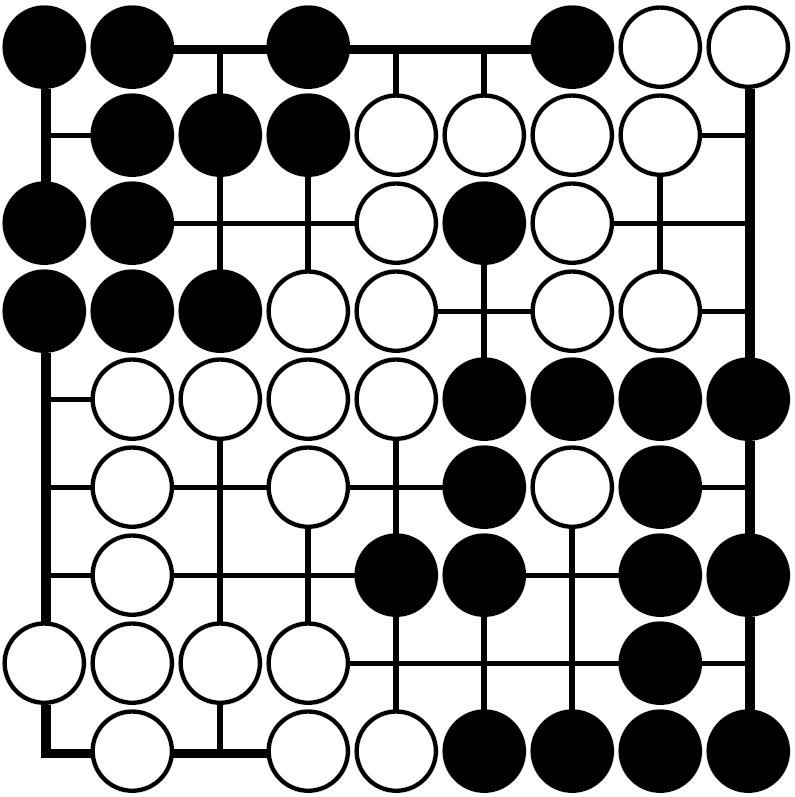
\includegraphics[width=.4\textwidth]{../img/late_endgame_Go_position_suited_for_exact_analysis.png}
  \captionWithCite{An~immortal wall enabling an exact analysis during late endgame}{Muller1995computer}
  \label{fig:immortal-wall}
\end{figure}
No move can have any influence across these ``immortal'' walls and significant parts of~the board definitely belong to one of the players.
The connected components of~remaining stones define local subgames independent from each other.

In the opening and midgame, only approximate partitioning can be available.
In the endgame, conversely, the partition gets more precise:
the status of~all big groups has been settled, and the outlines of~territories are clear.
If each local game is simple enough to~analyze completely (such as in Figure~\ref{fig:immortal-wall}), combinatorial game theory can compute an~optimal move for the full board position.
(\cite{Muller1995computer})

This is the general procedure of~(\cite{Muller1995computer}) for playing Go as a~sum of~local games:
\begin{enumerate}
  \item Board partition: find safe blocks, safe territories, and local areas.
  \item Generate local game trees in each area.
  \item Evaluate local terminal positions.
  \item Transform local game trees into mathematical games (and simplify games).
  \item Find an optimal move in the (combinatorial game theory) sum-game and play it.
\end{enumerate}
\Mueller{} proposes heuristic algorithms for playing the entire game, and exact algorithms for late endgame positions.

Undoubtedly, the task of~solving endgames in 1995 (at the age of Computer Go's infancy) already played a~vital role.

\subsection{Combinatorial Game Theory and Sum-Game Model for Approximate Play}

\epigraph{
  [$\dots$]
  You get surreal numbers by playing games.
  I used to feel guilty in Cambridge that I spent all day playing games, while I was supposed to be doing mathematics.
  Then, when I discovered surreal numbers, I realized that playing games IS math.
}{John Horton Conway}

\Mueller{} suggests to replace the ``standard model'' of~computer Go by a~sum-game model.
Here follows some of~the general benefits and problems of~the sum-game model for computer Go as listed in~(\cite{Muller1995computer}):

\medskip

\underline{Benefits}
\begin{itemize}[+]
  \item suitability to the knowledge and style of~Go programs at that time:
    local fighting, surrounding territories$\dots$
  \item the reuse of~local game analysis for higher quality game-play
  \item simplification of~move generation and position evaluation.
  \item translation of~Go terms into the theory, without any need to separate programming
  \item opportunities for parallelism:
    independent local searches, evaluation and operations on mathematical games$\dots$
\end{itemize}

\underline{Problems}
\begin{itemize}[-]
  \item required accurate board partition and recognition of~dependencies
  \item the common issues of~selective search:
    misleading evaluation due to missing crucial moves in~complicated games
  \item the lack of~long-range full-board planning:
    ``This is probably not a~big issue until programs reach amateur Dan or even professional level.''%
    \footnote{For an~update on the situation today, see Section~\ref{sec:AlphaGo}.}
\end{itemize}

\subsection{Board Partition and Subgame Dependencies}
\epigraph{
  Independence?
  That's middle class blasphemy.
  We are all dependent on~one another, every soul of~us on Earth. 
}{George Bernard Shaw}
In addition, (\cite{Muller1995computer}) mentions several further obstacles of~the sum-game model, caused by~the heuristic board partition:

\begin{itemize}[-]
  \item the impossibility of a~perfect, precise split:
    During the opening or~midgame, there are almost no surrounded spaces, and moreover, the surrounding stones would not be invulnerable yet.
    Heuristics is needed for board partition to split the imperfectly surrounded areas.

  \item the infeasibility of~exhaustive search in still large subgames:
    The program is obliged to give a~move in a~few seconds or minutes.
    However, there still remain areas intractable for an~exhaustive search.

    In such subgames, \Mueller{} employs \emph{selective search} method.
    He limits the number of~generated moves and stops the search before reaching a~terminal position.
    For each local game, nodes to expand need to be decided and \emph{expert modules for search and evaluation} need to be selected.
    A~post-processing stage handles detected dependencies between games.

  \item the dependencies between the resulting subgames, which arise with the previously mentioned heuristics:
    The effect of~such dependencies differs widely:
    often it is so small that independence is a~useful approximation.
    In cases when a~move works as a~\emph{double threat} however, dependency analysis is crucial.

    Trivial strategies to overcome dependencies involve:
    \begin{itemize}
      \item ignoring the dependency, as if the games were independent,
      \item proving that the dependency does not affect the value of~the sum, or play of~the sum game,
      \item merging mutually dependent local games, then re-search the combined game, possibly using previously generated information on single games,
      \item analyzing the interaction between local games, then use a~specialized theory to compute the joint game value.
    \end{itemize}
\end{itemize}

Hence, the sum game model makes the best sense during the endgame part.
This general principle is as well applicable in poker:
we wait until the late stage of~the game, when it has greater impact to refine and re-solve the reached endgames.

\subsection{Local Search and Evaluation in the Endgame}
\epigraph{
  True genius resides in~the capacity for~evaluation of~uncertain, hazardous, and conflicting information. 
}{Winston Churchill}

Once the board is partitioned, the algorithm of~(\cite{Muller1995computer}) for converting a~Go endgame into a~combinatorial game follows these steps:
\begin{enumerate}
  \item Generate local game trees:
    all legal moves are generated from point of~both players, with exceptions~of:
    \begin{enumerate}[(a)]
      \item \emph{pruning rules}%
        \footnote{Compare with \emph{policy networks} of~AlphaGo in Section~\ref{sec:AlphaGo}.},
        e.g. pruning dominated subgame trees:
        the evaluation of~nodes allows for pruning moves dominated by other moves.
        Moves with a~dominating alternative are labelled as~\emph{locally bad moves}.

      \item \emph{termination rules} for static evaluation of a~position, without further tree expansion%
        \footnote{Compare with \emph{value network} of~AlphaGo in Section~\ref{sec:AlphaGo}.}
    \end{enumerate}

  \item Score local terminal positions:
    \begin{enumerate}[(a)]
      \item \emph{scoring}%
        \footnote{See Section~\ref{sec:Go}.}
        comes in two widely-accepted flavors, namely
        \begin{enumerate}[$\diamondsuit$]
          \item Chinese variant, which counts stones and empty points belonging to either color,
          \item Japanese variant, which counts territory and prisoners.
        \end{enumerate}
        Both variants have straightforward implementation because safe stones, dead stones, territories and neutral points are known exactly in~the endgame.

      \item \emph{terminal positions} can be recognized by
        \begin{enumerate}[$\diamondsuit$]
          \item no more legal moves,
          \item no more good moves,
          \item the value of~position already known from the transposition table, pattern, or local position database.
        \end{enumerate}
        A~position is additionally considered terminal, once we can ascertain its value from another source.
        Such a~value can be any value in~the sense of~mathematical games.

        Non-terminal positions may have a~constant value as well, if the outcome is the same no matter who plays first, but this has to be proven using search.
    \end{enumerate}

  \item Evaluate local games as mathematical games.
    Explicitly, evaluate terminal positions, and back up the values in~the tree, resulting in a~mathematical-game evaluation of~each node.

    Even though the program reaches a~solved position, (\cite{Muller1995computer}) notes that a~``suicidal'' opponent may later cause great troubles, by endangering his immortal stones.
    Such an~act would violate the assumptions on~board partitioning and give rise to~new unexpected positions with rather complicated optimal play.

  \item Select an~option in the resulting (abstract) sum-game.
  \item Translate the chosen option in~the abstract game into a~corresponding move in~Go.
    This move is taken as~the first move with sufficient \emph{incentive} (recall Section~\ref{sec:CGT}).
\end{enumerate}

\begin{figure}[H]
  \centering
  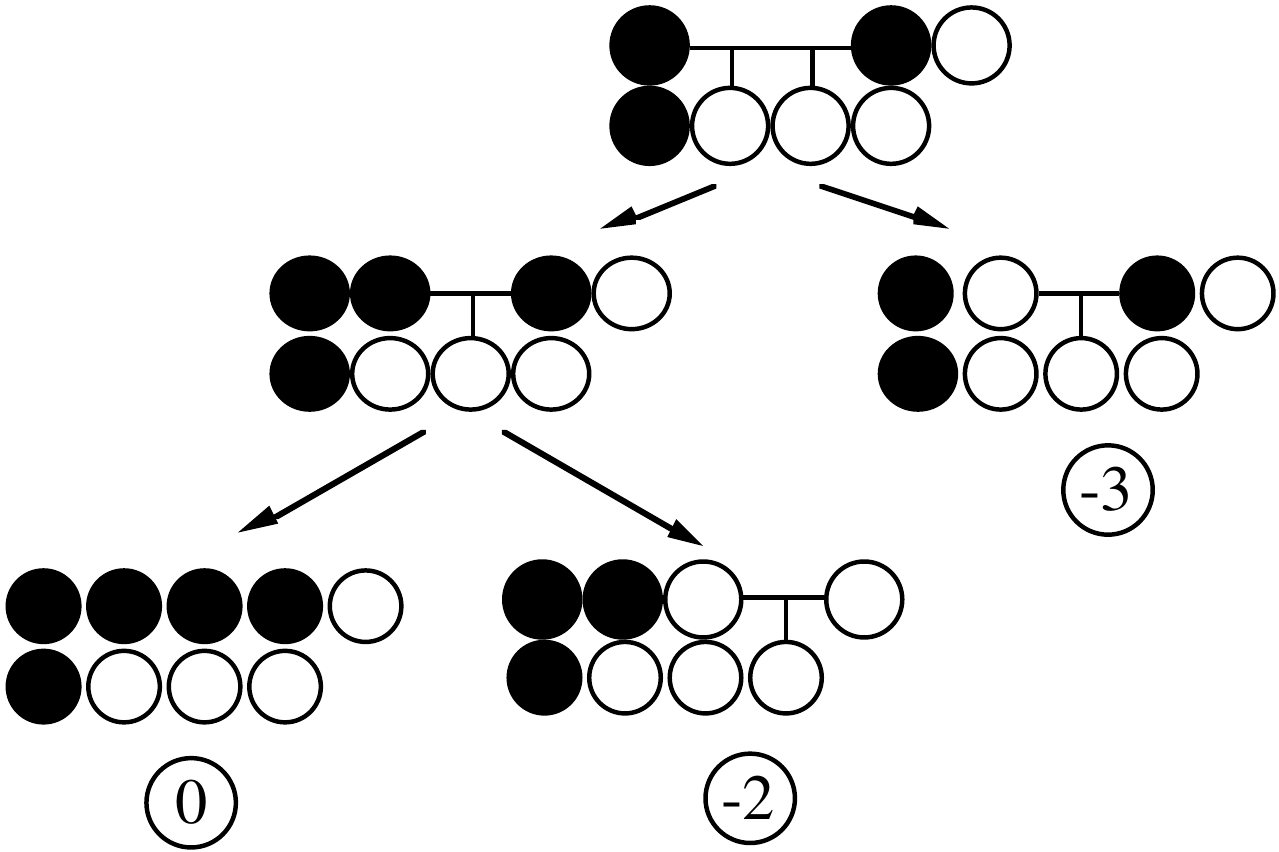
\includegraphics[width=.7\textwidth]{../img/Go_search_tree.png}
  \captionWithCite{Local game tree with evaluation of terminal nodes}{Muller1995computer}
\end{figure}

Search and analysis produce the complete description of possible endgame plays, facilitating the perfect strategy.
The results are stored in a~\emph{database of~local positions}.
Local subgames during a~live play are then matched one-to-one to a~set of~database positions.
The value of a~full board position is the sum of~local position values and an~algorithm for sum-game evaluation selects the best available response.

A~version with lower memory requirements is implemented as well.
This is achieved by~saving only a~selection of~positions, and in~case the subgame is missing in the database, re-doing the search.

An~important question is what to store.
Table~\ref{tab:db-loc-games} lists some possible answers:
\begin{table}[!htbp]
  \centering
  \begin{tabular}{ |p{.45\textwidth}|p{.48\textwidth}| } 
    \hline
    \textbf{Type of database} & \textbf{Content} \\
    \hline
    Full                            & $\dots$every position discovered during exhaustive search \\
    Color-complete (Black or White) & $\dots$every position reachable by~non-dominated moves of~the color and arbitrary opponent's moves (pruned bad moves of~the color) \\
    Optimal                         & $\dots$at~least one position corresponding to~every non-dominated option of~every reachable position (guarantees optimal play from every position in~database) \\
    Sufficiently good               & $\dots$guaranteed optimal score from a~starting position (might fail to exploit some opponent mistakes) \\
    \hline
  \end{tabular}
  \captionWithCite{Possible database variants of~local games}{Muller1995computer}
  \label{tab:db-loc-games}
\end{table}

One needs to make a~trade-off between re-computation time and storage space.
A~sensible solution is to~store only complicated moves in~the database, and re-calculate the rest when necessary.
It is a~good idea to save only the information whether a~move is locally good or bad, but discard \emph{refutations}\footnotemark.
\footnotetext{the trees proving that bad moves are inferior}
Such a~type of~database is robust against a~good opponent;
however, it suffers from a~play of a~locally bad opponent.
This~rare situation would call for the re-computation of~a~subtree in order to find a~refutation.

\subsection{Speeding up Local Search}

(\cite{Muller1995computer}) considers various improvements to computational efficiency:
\begin{quotation} \noindent
  Ignoring illegal moves and captures, the number of possible plays in an $n$ point area is approximately $2n$ ($n$ for each player), and play generates a $n-1$ point area.
  A~rough estimate for the size of~the game tree is therefore $2n\cdot2(n-1)\cdot \ldots \cdot2 = 2^n n!$

  Due to this combinatorial explosion, even fairly small endgames become prohibitively expensive to compute using this approach.
  In the following, we look at a~number of~techniques for reducing the size of the search tree.
\end{quotation}

\begin{enumerate}[(a)]
  \item transposition table (see also Table~\ref{tab:reduction-transp-tab})
    \begin{quotation} \noindent
      A~transposition table detects identical board positions, reducing the size of~the search space from $\approx 2^n n!$ to $3^n$ states.

      \begin{table}[!htbp]
        \centering
        \begin{tabular}{ |rrr| }
          \hline
          \textbf{$n$} & \textbf{$2^nn!$} & \textbf{$3^n$} \\
          \hline
          1	&	2	&	3 \\ 
          2	&	8	&	9 \\ 
          3	&	48	&	27 \\ 
          4	&	384	&	81 \\ 
          5	&	3840	&	243 \\ 
          6	&	46080	&	729 \\ 
          7	&	645120	&	2187 \\ 
          8	&	10321920	&	6561 \\ 
          9	&	185794560	&	19683 \\ 
          10	&	3715891200	&	59049 \\ 
          \hline
        \end{tabular}
        \caption{Reduction of search space by transposition table}
        \label{tab:reduction-transp-tab}
      \end{table}
    \end{quotation}

  \item pruning moves
    \begin{quotation} \noindent
      The width of~the search tree can be further reduced by pruning moves.
      In contrast to selective search, we may only eliminate moves that are provably worse-or-equal than others.
      If a~move achieves all points of~the local area, or if any other move would give the opponent an~answer which achieves the maximum score, the move is optimal, and we can prune all other moves.
    \end{quotation}
\end{enumerate}

\subsection{Using Combinatorial Game Theory to Solve Late Endgames by Computer}

These are some objectives that can be accomplished by the approach of~(\cite{Muller1995computer}):
\begin{itemize}
  \item Perfect computer play in late endgame
  \item Find the game-theoretic value of a position long before the end
  \item Evaluate the opponent’s endgame moves
  \item Find moves that are good enough even with a reduced local game database
\end{itemize}
On the other hand, the work also remarks that strict analysis of~endgames is not possible with this method if one of the following limits is reached:
\begin{itemize}
  \item \textbf{Partition:}
    too few blocks can be proven safe independent of~endgame play.
    Therefore some areas become too big for complete search.
  \item \textbf{Summation:}
    no move with dominating incentive exists, and both summing and partial search take too long.
  \item \textbf{Ko:}
    Standard combinatorial game theory exploits the independence of~local games.
    In the case of~Ko, the independence is broken (a~locally bad move may be globally best if it serves as a~Ko threat).
    Generalizations of~the theory to handle Kos are a topic of [at that time] current research.
  \item \textbf{Added complexity in ‘obvious’ situations:}
    In cases where the focus of~play is obvious (i.e. only one local situation is relevant), combinatorial game theory introduces additional complexity by investigating moves for both players in this and each other position.
\end{itemize}

\subsection{Time and Memory Management}

One reason why endgames are exhaustively studied is due to their computational benefits.
As the game progresses, more exact analysis can be done, and thus, time and memory resources may be better utilized.
In particular, (\cite{Muller1995computer}) uses following ``adaptive'' resource adjustments:

\begin{enumerate}[(a)]
  \item memory management of objects and local trees
    \begin{quotation} \noindent
      In a~program with limited memory, we need to decide which local game nodes and other calculated results to keep, and which to dispose during the course of play.
      Which items are obsolete, and which can probably be reused later?
      Only heuristic rules for memory management are possible, because the future actions of~the user are unpredictable.

      During the course of a~game there is a~gradual shift of~relevance.
      Starting a~new game leads to radical change, just about all computed results are useless in the new game.
      Some flexibility for users undoing moves should be provided.

      As a~solution we define a~\emph{forced substate}, a subset of all points on the current board.
      The substate consists mainly of~safe-looking stones.
      We delete all objects that do not match the forced substate.
      For supporting undo’s, we exclude all points affected by the last two moves from the points of~the forced substate.
      Some items are exempt from automatic disposal:
      user inputs, and objects explicitly calculated on a~user’s demand.
    \end{quotation}

    \parbox{.9\textwidth}{
    \item time control for tournament play
      \begin{quotation} \noindent
        Time control determines how much time to use for each subgame, for tactics, and for
        Life\&Death problems. [$\dots$]
        The same algorithm with smaller time slices could be used for computing in opponents time.
        A~fast mode is used in time trouble:
        only minimal time is used for subproblems such as tactics calculations and Life\&Death.
      \end{quotation}
    }

\end{enumerate}

\subsection{Pattern Learning}

Pattern recognition is one of~the key components of~AlphaGo (see Section~\ref{sec:AlphaGo}).
Arguably, the program's success might be partially attributed to learning Go patterns from human expert plays.
For comparison, (\cite{Muller1995computer}) reports the following state of~``Go-related Research in Visual Perception, Machine Learning and Neural Networks'' in 1995:
\begin{quotation} \noindent
  Go has been used as a~vehicle for research in~visual perception, machine learning and neural networks (\cite{Wilcox79}, \cite{Enderton1991golem}, \cite{Stoutamire1991machine}, \cite{Schraudolph1994temporal}).
  Starting from only the rules of~the game, learning programs can typically pick up basic Go principles, such as saving a~stone from capture, or making a~[one-point] jump.

  A~most disturbing fact is that since Wilcox’ pioneering efforts, none of~this research has been applied to a~state-of-the-art Go program.
  The problems of~automatically tuning and expanding an~existing knowledge base, or learning of~new high-level concepts, seem quite different from the ab-initio learning problems that have been researched.

  Low level concepts can be learned, but they have already been programmed in the better programs.
  Neural networks can be trained to play locally good shapes, but have no clue when to play it.%
  \footnote{This assertion, in particular, has changed with AlphaGo.}
  Such programs fall easy prey to those that know more about tactics and Life\&Death.
\end{quotation}
(\cite{Muller1995computer}) also suggests pattern matching as a~promising mean for improvement:
\begin{quotation} \noindent
  Research on pattern learning in computer Go has unfortunately been restricted to \emph{ab-initio} learning of~the most basic patterns from zero knowledge.
  Interactive or automatic tuning and expansion of a~state-of-the-art pattern base is another fascinating research topic.
\end{quotation}

\subsection{Contributions of~Combinatorial Game Theory to Go Endgames}

The doctoral thesis (\cite{Muller1995computer}) highlights following contributions to general computer science:
\begin{itemize}
  \item Scientists are fascinated by problems which can be stated simply, yet are hard to solve.
    Computer Go is a~prime example.
    We have brought the divide-and-conquer approach, a~fundamental paradigm of~computer science, to bear on computer Go.

  \item The application of a~sophisticated mathematical theory to computer Go provides an~example of~algorithms for a~nontrivial decomposition of a~complex problem.
\end{itemize}
Another contributions are the ones aiding computer Go endgames specifically:
\begin{itemize}
  \item We have implemented a~\emph{late endgame player}, a~niche where program play surpasses human play in both speed and exactness.
    We did this by applying concepts from combinatorial game theory to Go.
    The program plays a~wide variety of`late endgame positions perfectly.

  \item We have developed algorithms for board partition and dependency analysis.
    The central idea of~board partition has been used both in a~program following a~traditional model, and in a~program based on the sum game approach.
\end{itemize}
Hence, the work employs a~technique of~applying an~elaborate mathematical theory (of~combinatorial game theory) to deal with the endgame phase.
In particular, CGT is used to ``connect'' individual relevant subgames, which may be solved independently.

As we will see later, the situation in the case of~Poker is slightly more delicate:
the imperfect-information property prevents us from using an~immediate divide-and-conquer approach.
Instead, we will \emph{augment} the information by saturating it with additional game states (see Section~\todo).

\note{
  \label{note:CGTvsAlphaGo}
  It is also interesting to compare the method of~(\cite{Muller1995computer}) with the modern approach of~\emph{AlphaGo}:
  the ad-hoc Go-specific knowledge is replaced with general-learning neural networks and the probabilistic \emph{Monte Carlo Tree Search} algorithm.
  Such a~combination has the capability to surpass professional human players at the highest ranks.
  On top of that, this solution can be adapted to other games without substantial modifications.
  As long as there is an~abundance of~available data, the system can always be trained with no need to imbue it with any game-specific knowledge.
  See Section~\ref{sec:AlphaGo} for more details.
}

\section{Go Endgames Using Neural Networks}
\label{sec:AlphaGo}

As of~today, over 20 years have passed since \Mueller's work.
\emph{DeepMind}, a~London-based AI start-up recently acquired by Google, has developed the strongest computer Go program so far:
\emph{AlphaGo}.

This section is based on~the article ``Mastering the game of Go with deep neural networks and tree search''~(\cite{Silver2016mastering}), which documents the internals of~AlphaGo:

\begin{quotation} \noindent
  The game of~Go has long been viewed as~the most challenging of~classic games for artificial intelligence owing to its enormous search space and the difficulty of~evaluating board positions and moves.

  Here we introduce a~new approach to computer Go that uses \emph{value networks} to evaluate board positions and \emph{policy networks} to select moves.
  These deep neural networks are trained by a novel combination of supervised learning from human expert games, and reinforcement learning from games of self-play.
  Without any lookahead search, the neural networks play Go at the level of~state-of-the-art Monte Carlo tree search programs that simulate thousands of~random games of~self-play. 

  We also introduce a~new search algorithm that combines Monte Carlo simulation with value and policy networks.
  Using this search algorithm, our program AlphaGo achieved a~99.8~\% winning rate against other Go programs, and defeated the human European Go champion by 5 games to~0.
  This is the first time that a~computer program has defeated a~human professional player in the full-sized game of~Go, a~feat previously thought to be at least a~decade away.
\end{quotation}
For more details, also consult my presentations on AlphaGo given at:
\begin{itemize}
  \item Spring School of Combinatorics 2016 (Charles University in Prague): \\
    \href{http://www.slideshare.net/KarelHa1/mastering-the-game-of-go-with-deep-neural-networks-and-tree-search-presentation}
    {\tt http://www.slideshare.net/KarelHa1/mastering-the-game-of-go\\-with-deep-neural-networks-and-tree-search-presentation}

  \item Optimization Seminar (Charles University in Prague) \\
    \href{http://www.slideshare.net/KarelHa1/alphago-mastering-the-game-of-go-with-deep-neural-networks-and-tree-search}
    {\tt http://www.slideshare.net/KarelHa1/alphago-mastering-the-game\\-of-go-with-deep-neural-networks-and-tree-search}

  \item Distributed Computing group (ETH \Zurich) \\
    \href{http://www.slideshare.net/KarelHa1/alphago-for-disco-group-of-eth-zurich}
    {\tt http://www.slideshare.net/KarelHa1/alphago-for-disco-group\\-of-eth-zurich}
\end{itemize}

\subsection{Game-Tree Search}

Optimal value~$v^*(s)$ determines the~outcome of~the game from every board position $s$ under perfect play by~all players.
This value can be computed by~recursively traversing the~search tree containing approximately $b^d$ possible sequences of moves, where $b$ is the breadth of~game (number of legal moves per position) and $d$ is its depth (game length).

In~the case of~chess, that is $b \approx 35$ and $d \approx 80$, whereas Go has $b \approx 250$ and $d \approx 150$.
This amounts to a~terrifying overnumerousness: there are more Go positions than atoms in the observable Universe.
Furthermore, ``that makes Go a~googol [$10^{100}$] times more complex than chess'',%
\footnote{\href{https://deepmind.com/alpha-go.html}{https://deepmind.com/alpha-go.html}}
and therefore, exhaustive search is deemed intractable.

How to handle the size~of the game tree? For the$\dots$
\begin{itemize}
  \item $\dots$breadth: we train a~neural network to~select moves.
  \item $\dots$depth: we train a~neural network to~evaluate the current position.
  \item $\dots$tree traverse: we use Monte Carlo tree search method.
\end{itemize}

\textbf{Monte Carlo tree search} (MCTS) is a~Monte Carlo heuristic of~the classical tree search.
However, instead of traversing the entire game tree, the MCTS selects the~most promising moves, expanding the search tree based on~random sampling.

In~each iteration, the game is played-out to~the very end by~choosing moves at~random.
The final outcome of~each playout is then used to~weight the nodes in~the game tree accordingly.
Thus, better nodes are more likely to be chosen in future playouts.

\begin{figure}[H]
  \centering
  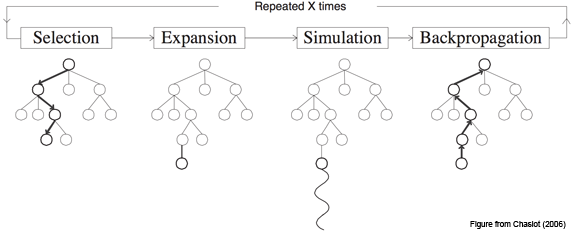
\includegraphics[width=.6\textwidth]{../img/MCTS.png}
  \caption{The scheme of~MCTS}
  \label{fig:MCTS}
\end{figure}

\subsection{Neural networks}

Inspired by biological neural networks, an~artificial neural network (ANN) is a~network of~interconnected nodes that make up a~model.
ANNs can be defined as~statistical learning models that are used to approximate functions which depend on a~large number of~inputs.
Neural networks are typically used when the volume of~inputs is far too large for~standard machine learning approaches.

\begin{figure}[H]
  \centering
  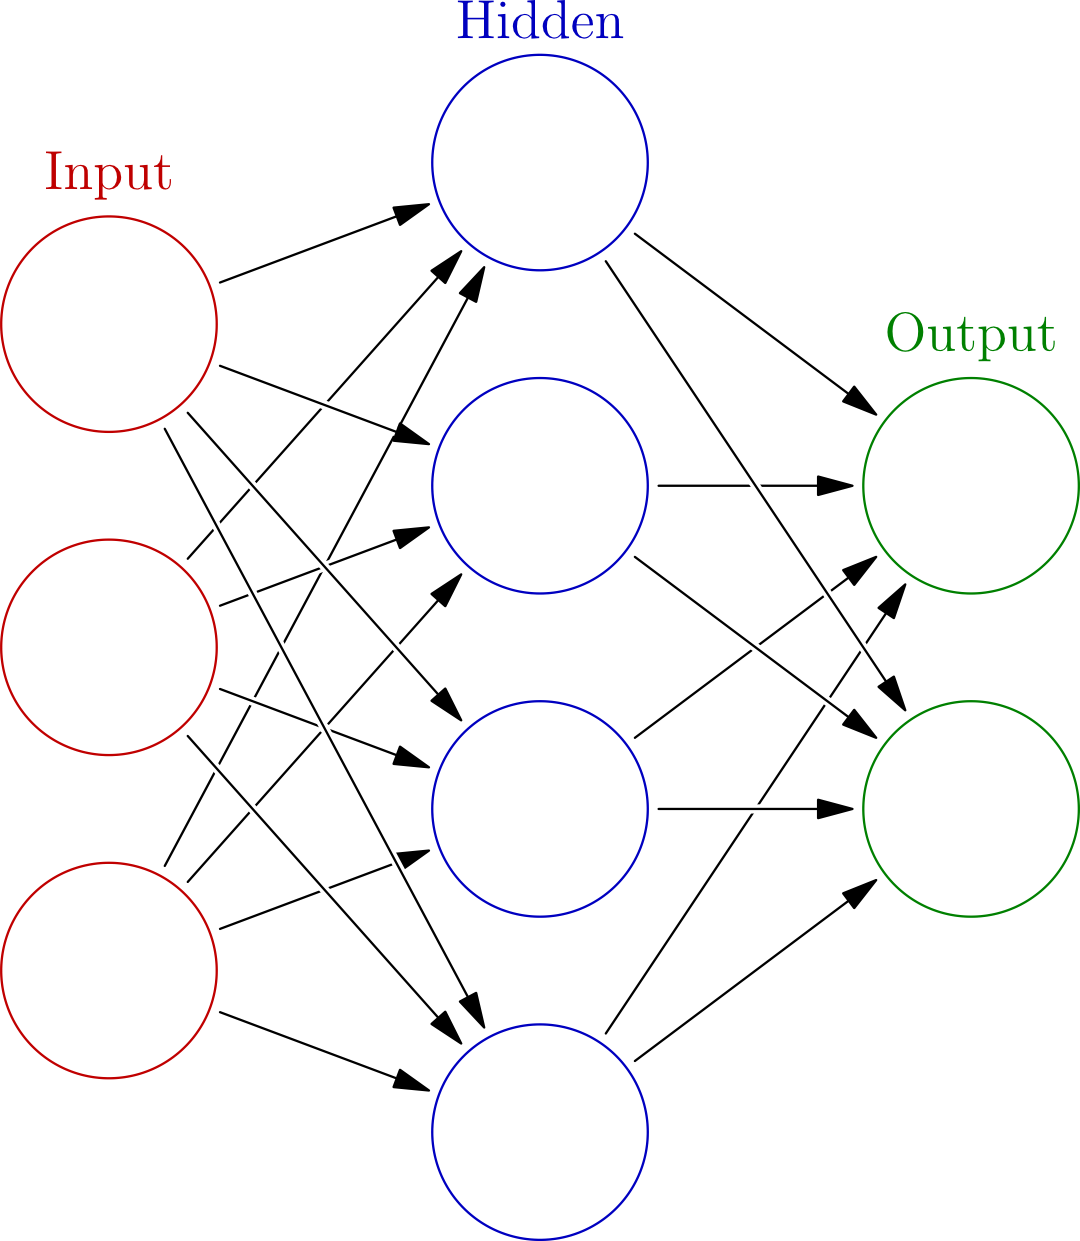
\includegraphics[height=.2\textheight]{../img/colored_neural_network.png}
  \caption{A~shallow neural network with 3 layers}
  \label{fig:shallow-neural-network}
\end{figure}

\textbf{Convolutional neural network} (CNN) is a~neural network suitable for high-dimensional inputs (e.g. a~large number of~pixels in an~image).
CNNs are frequently used in~computer vision (for identifying objects in an~image, for face detection in~photos etc.).
They are invariant to expectable transformations of~input, such as translations of~objects in~a~picture or changes in~illumination.

\textbf{Deep neural network} (DNN) is a~neural network with many hidden layers.
It can model complex non-linear relationships, e.g. in~speech, in~images, in~videos or in~board positions of~Go.

\subsection{Pipeline of Neural Networks}

AlphaGo employs two kinds of deep convolutional neural networks---a~\emph{policy network} (for move selection) and a~\emph{value network} (for board evaluation).
\begin{figure}[H]
  \centering
  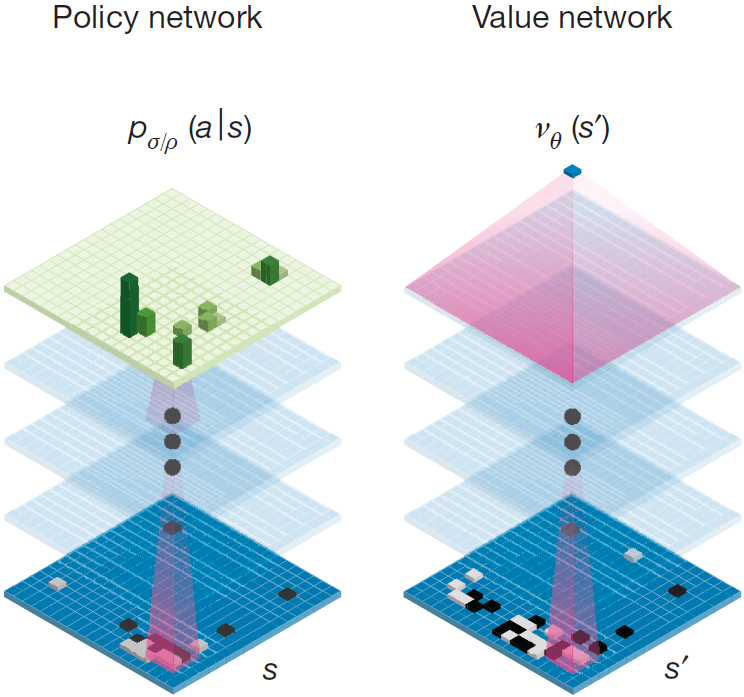
\includegraphics[width=.5\textwidth]{../img/policy_and_value_network.png}
  \captionWithCite{Comparison between policy and value network}{Silver2016mastering}
  \label{fig:policy_vs_value_nets}
\end{figure}

In the following Figure~\ref{fig:neural_nets_pipeline}, we can view the whole training process of~AlphaGo's neural networks.
\begin{figure}[H]
  \centering
  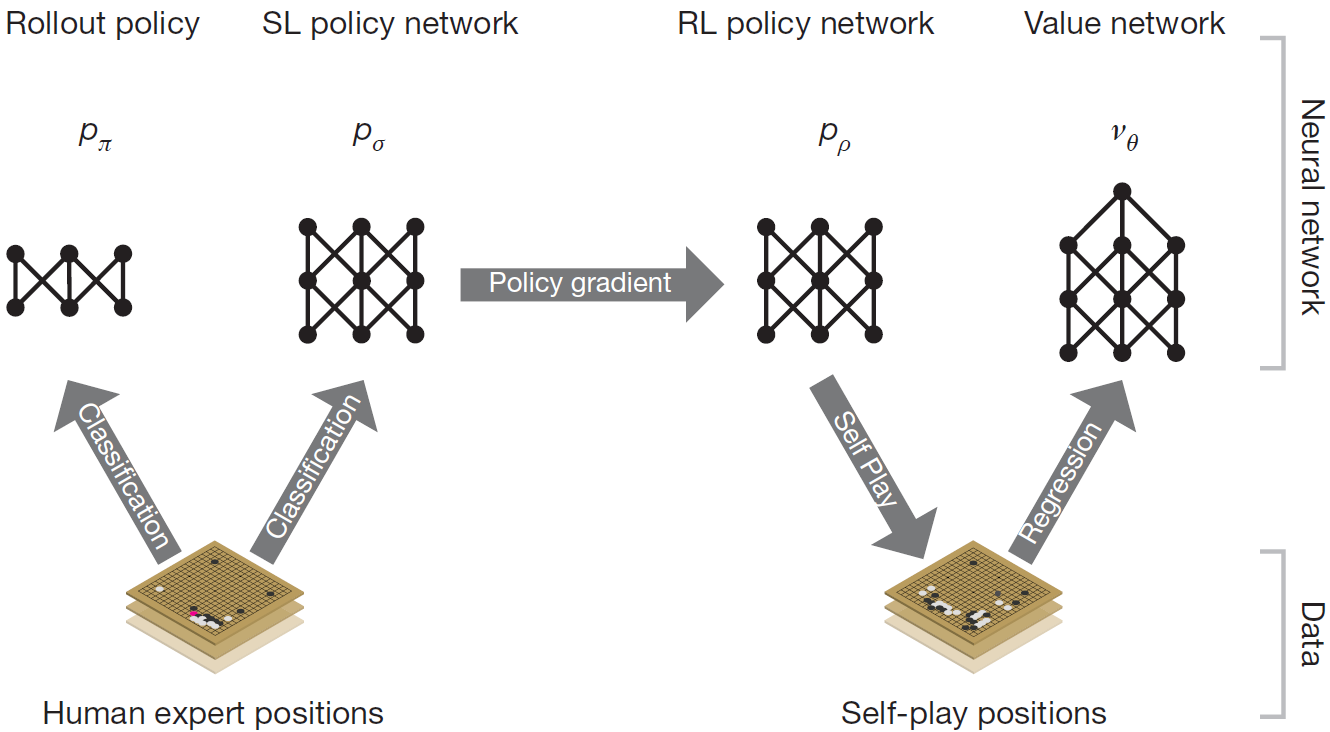
\includegraphics[width=.7\textwidth]{../img/neural_nets_pipeline.png}
  \captionWithCite{Training the neural networks of~AlphaGo: the~pipeline~and~the~architecture}{Silver2016mastering}
  \label{fig:neural_nets_pipeline}
\end{figure}

\textbf{Rollout policy} $p_\pi$ is a~CNN rapidly sampling actions during a~\emph{rollout} (a~fast-forward simulation from a~position to the end of~the game).
It predicts expert human moves much faster but less accurately than $p_\sigma$ (see below).
The output is a~probability distribution over all moves.

\textbf{Policy network} is a~CNN selecting moves.
It addresses the problem of the game-tree breadth.
There are two flavors of~these networks:
\begin{itemize}
  \item \textbf{SL policy network} $p_\sigma$ is trained by \underline{s}upervised \underline{l}earning to predict expert human moves.
  \item \textbf{RL policy network} $p_\rho$ is trained by \underline{r}einforcement \underline{l}earning to win in the~games of~self-play.
\end{itemize}

\textbf{Value network} $v_\theta$ is a~CNN evaluating board positions, so as to address the problem of the game-tree depth.
It is trained by regression to predict the outcome in~positions of~the self-played games.

\subsection{Main Algorithm}

Finally, the neural networks are combined with MCTS into the main algorithm.

During the play, AlphaGo simulates up to 100 possible continuations per each move by selecting the most promising actions and following them.
This way, it descends the game-tree down to a~depth given by a~parameter.
At that point, leaf nodes are evaluated in two ways:
\begin{enumerate}[(1)]
  \item using the dedicated value network $v_\theta$,
  \item simulating the self-play until the terminal positions, using the fast rollout policy $p_\pi$.
\end{enumerate}
The two are mixed into the final value of~the leaf node.

Once every simulation of a~single round is finished, all new values are backpropagated to the root, thus updating necessary variables on the way up.

For more details, consult (\cite{Silver2016mastering}) or the before-mentioned presentations.

\note{
  Main algorithm demonstrates the connection to \emph{our theme of~endgames}:
  the simulations may be viewed as ``solving endgames''.
  In particular, the $p_\pi$ rollouts somehow remind of~exhaustive search for the game value during the late stage of~the play.
  In this sense, the approaches of~AlphaGo and endgame computation bear a~striking similarity.

  On the other hand, AlphaGo performs the same simulation algorithm during the whole game:
  from an~empty board until the final move.
  Therefore, it would be imprecise to talk about ``endgame'' here.
}

\subsection{Playing Strength}

In order to assess the playing strength of~AlphaGo, DeepMind has organized an~internal tournament between different other Go programs,%
\footnote{\emph{CrazyStone} and \emph{Zen} are the strongest commercial programs, whereas \emph{Pachi} and \emph{Fuego} are strongest among the open-source ones.}
as well as a~duel of~AlphaGo against the European Go Champion Fan Hui.
Figure~\ref{fig:Go-tournament} displays the outcome of the tournament:

\begin{quotation} \noindent
  Each program used approximately 5 s computation time per move.
  To provide a~greater challenge to AlphaGo, some programs (pale upper bars) were given four handicap stones (that is, free moves at~the start of~every game) against all opponents.
  Programs were evaluated on an Elo scale: a~230 point gap corresponds to a~79\% probability of winning, which roughly corresponds to one amateur dan rank advantage on KGS;
  an~approximate correspondence to human ranks is also shown, horizontal lines show KGS ranks achieved online by that program.
  Games against the human European champion Fan Hui were also included;
  these games used longer time controls.
  95\% confidence intervals are shown.~(\cite{Silver2016mastering})
\end{quotation}

\begin{figure}[H]
  \centering
  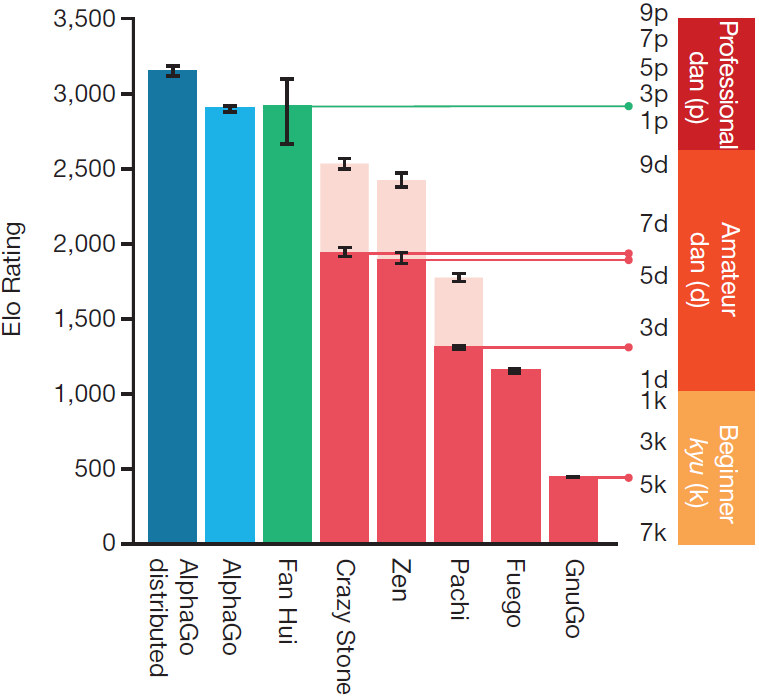
\includegraphics[width=.5\textwidth]{../img/results_of_tournament.png}
  \captionWithCite{Tournament with other programs and Fan Hui}{Silver2016mastering}
  \label{fig:Go-tournament}
\end{figure}

Here is an~official report provided by Google DeepMind%
\footnote{\href{https://deepmind.com/alpha-go.html}{https://deepmind.com/alpha-go.html}}
about AlphaGo's matches against human professionals:
\begin{quotation} \noindent
  After our program AlphaGo won 5--0 in a~formal match on~October 2015, against the reigning 3-times European Champion, Fan Hui, becoming the first program to ever beat a~professional Go player in an~even game;
  AlphaGo then went on to complete its ultimate challenge.

  In March 2016 AlphaGo won 4--1 against the legendary Lee Sedol, the top Go player in the world over the past decade.
  The matches were held at the Four Seasons Hotel, Seoul, South Korea on March 9\textsuperscript{th}, 10\textsuperscript{th}, 12\textsuperscript{th}, 13\textsuperscript{th} and 15\textsuperscript{th} and livestreamed on DeepMind’s YouTube channel as well as broadcast on TV throughout Asia through Korea’s Baduk TV, as well as in China, Japan, and elsewhere.

  They were played under Chinese rules with a~komi of~$7.5$ (the compensation points the player who goes second receives at~the end of~the match).
  Each player received two hours per match with three lots of 60-second byoyomi (countdown periods after they have finished their allotted time).
\end{quotation}

Following from this, computers seem to have reached the ``superhuman'' level of~expertise and they now appear to be superior to humans in~the game of~Go.
